\documentclass{article}
\usepackage{amsmath}
\usepackage{amssymb}
\usepackage{graphicx}
\usepackage{hyperref}
\usepackage[version=4]{mhchem}

\title{Example 3}
\date{}

\begin{document}
\maketitle

As shown in the figure, circles \(O\) and \(P\) have radii 3 and 6, and are externally tangent. Points \(A\) and \(B\) are on the circle \(O\), and points \(C\) and \(D\) are on the circle \(P . A D\) and \(B C\) are common external tangents to both circles. Find the area of trapezoid \(A O P D\).\\
(A) \(54 \sqrt{2}\)\\
(B) \(27 \sqrt{2}\)\\
(C) 54\\
(D) \(54 \sqrt{3}\)\\
(E) \(18 \sqrt{3}\)\\
\centering
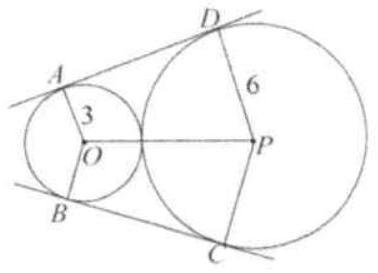
\includegraphics[width=\textwidth]{images/problem_image_1.jpg}

Solution: (B).\\
We draw a line through \(O\) parallel to \(A D\) intersecting \(P D\) at \(F\). So \(A O F D\) is a rectangle and \(O P F\) is a right triangle. \(D F\) \(=3, F P=3\), and \(O P=3+6=9\).\\
\centering
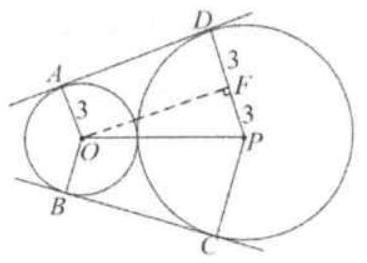
\includegraphics[width=\textwidth]{images/reasoning_image_1.jpg}

Applying Pythagorean Theorem to triangle \(O P F\) :\\
\(O F^{2}+F P^{2}=O P^{2} \Rightarrow O F^{2}=O P^{2}-+F P^{2}=81-9=72 \quad \Rightarrow O F=\sqrt{72}=6 \sqrt{2}\).\\
The area of trapezoid \(A O P D\) is \(12 \frac{(3+6) \times 6 \sqrt{2}}{2}=27 \sqrt{2}\).


\end{document}
